\section{Réflexions et réfractions sur le diamant}

Ici, le but était de trouver différentes méthodes de calculs de réflexion afin
d'être le plus proche de la réalité possible.

Une première approche simpliste mais
rapide à mettre en œuvre était l'utilisation d'une texture cubique. Cette méthode
est très rapide et permet un rendu de qualité raisonnable pour des objets simples.
Or, les diamants comportant des réflexions internes, cette méthode n'était pas très
convaincante. Un rendu cubique autour de chaque face pouvant apporter des artefacts
visuels sur des faces adjacentes et proches.

Nous avons donc creusé dans une autre direction. Le but est de générer,
pour chaque triangle de la scène,
un rendu de son monde «~miroir~» dans un buffer commun à toute la scène.

Voici le but recherché~:

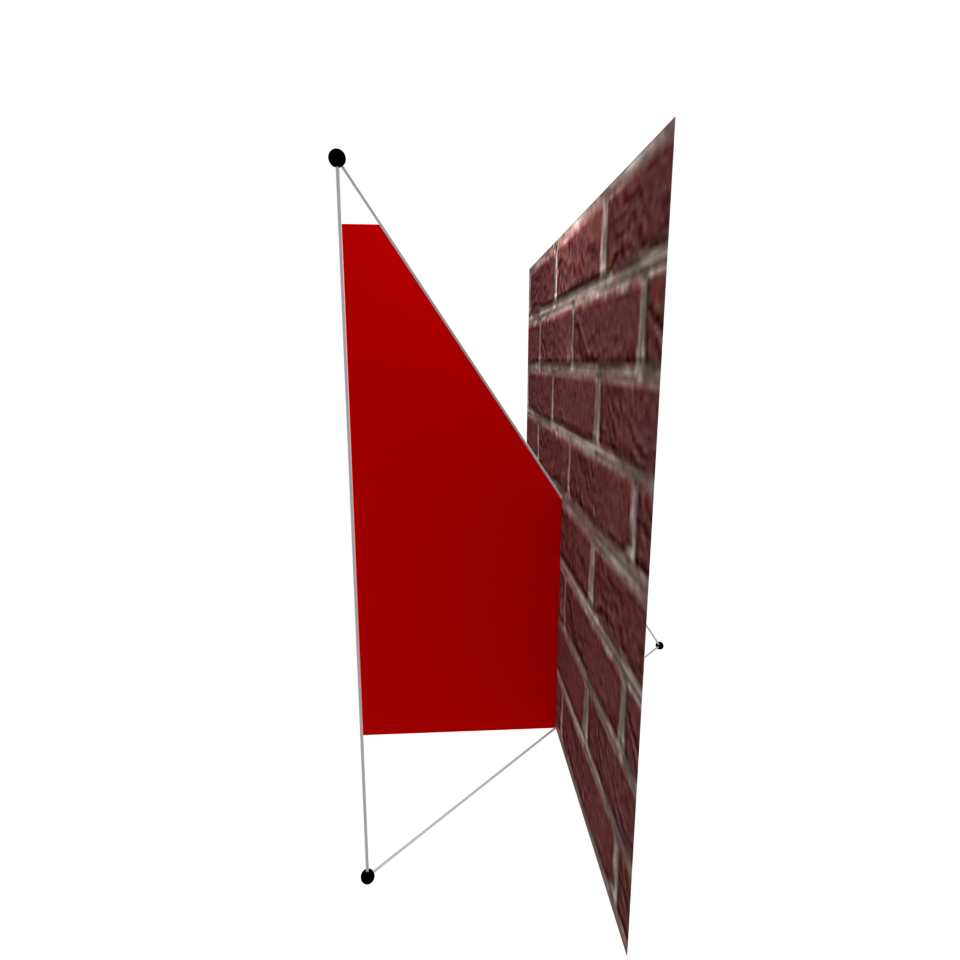
\includegraphics[width=0.45\textwidth]{Reflexion/6}

avec en rouge la zone où le rendu de la réflexion sera effectué.

Nous avons dans cet exemple, un carré, et un miroir triangulaire tourné à 45°.

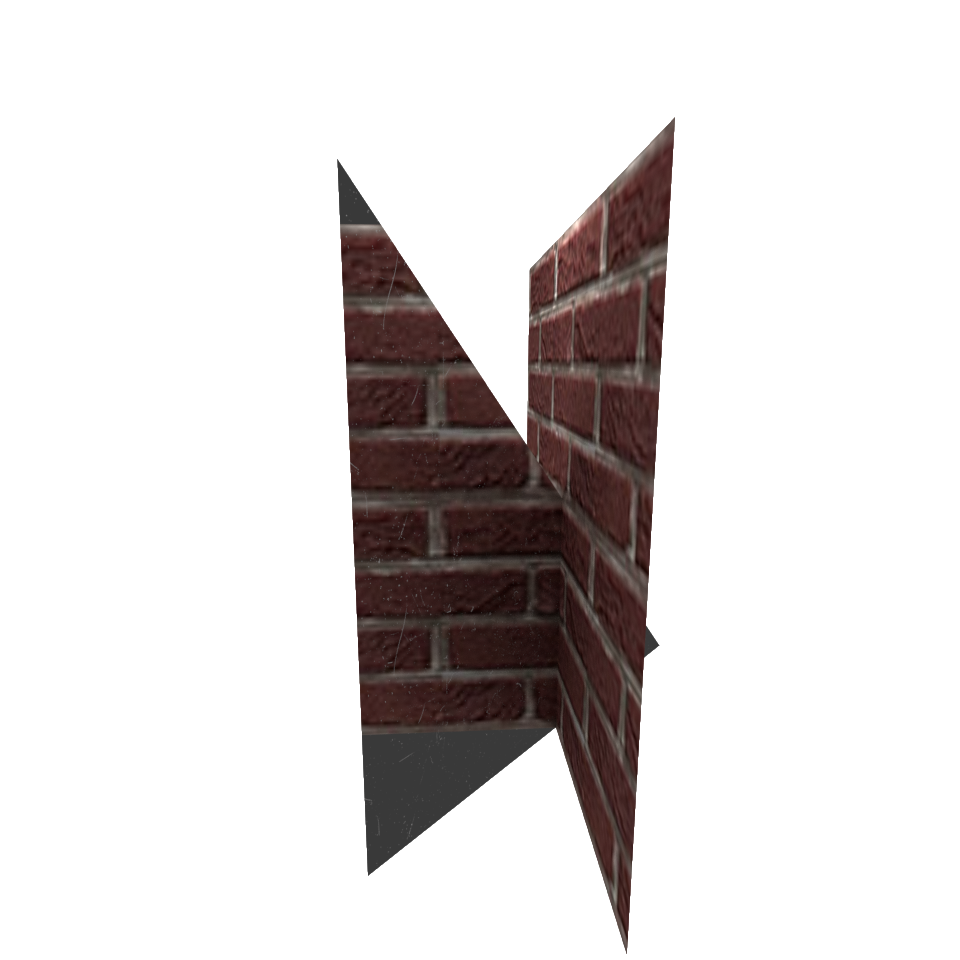
\includegraphics[width=0.45\textwidth]{Reflexion/1}

Pour chaque triangle se comportant comme un miroir~:

\begin{itemize}
    \item On récupère sa matrice Tangente - Bitangente - Normale (TBN) afin
        d'effectuer la réflexion de la scène par rapport a ce triangle.

        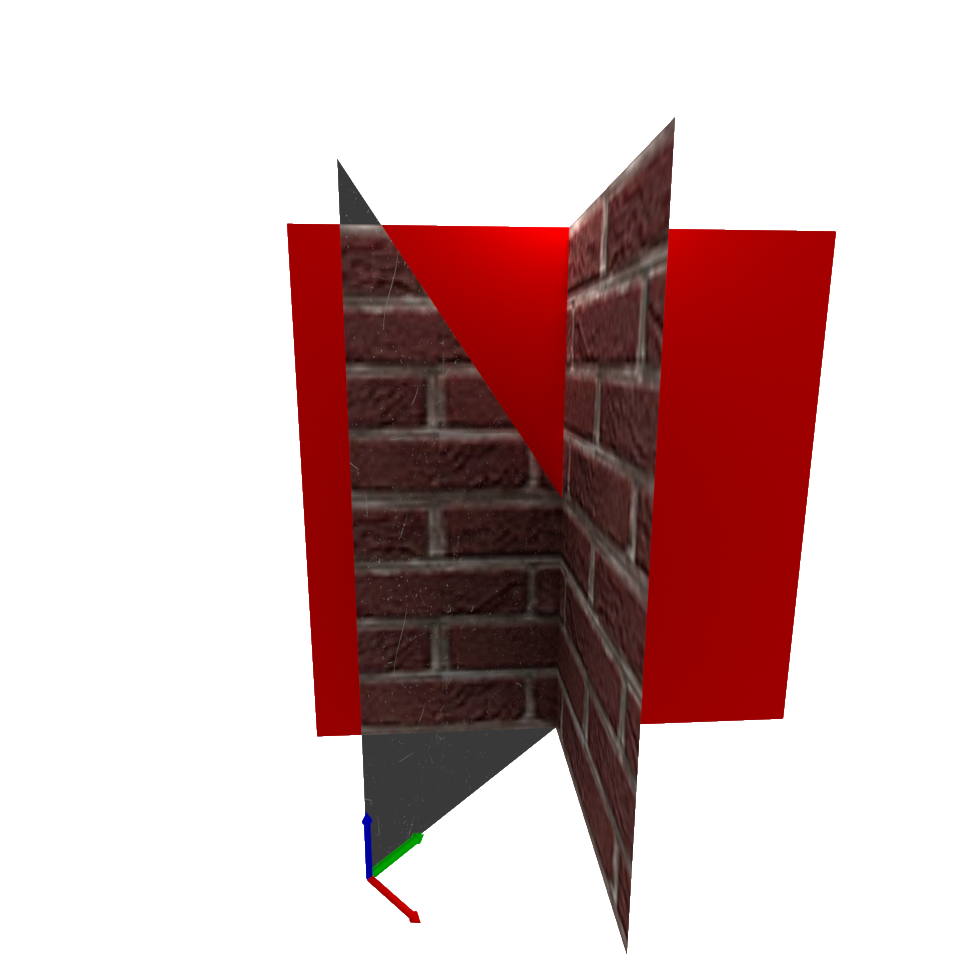
\includegraphics[width=0.45\textwidth]{Reflexion/3}

    \item On supprime ce qui se trouve derrière le carré de mur, étant donné qu'une
        fois la réflexion effectuée, c'est uniquement ce qui se trouve devant qui
        représente le reflet.

        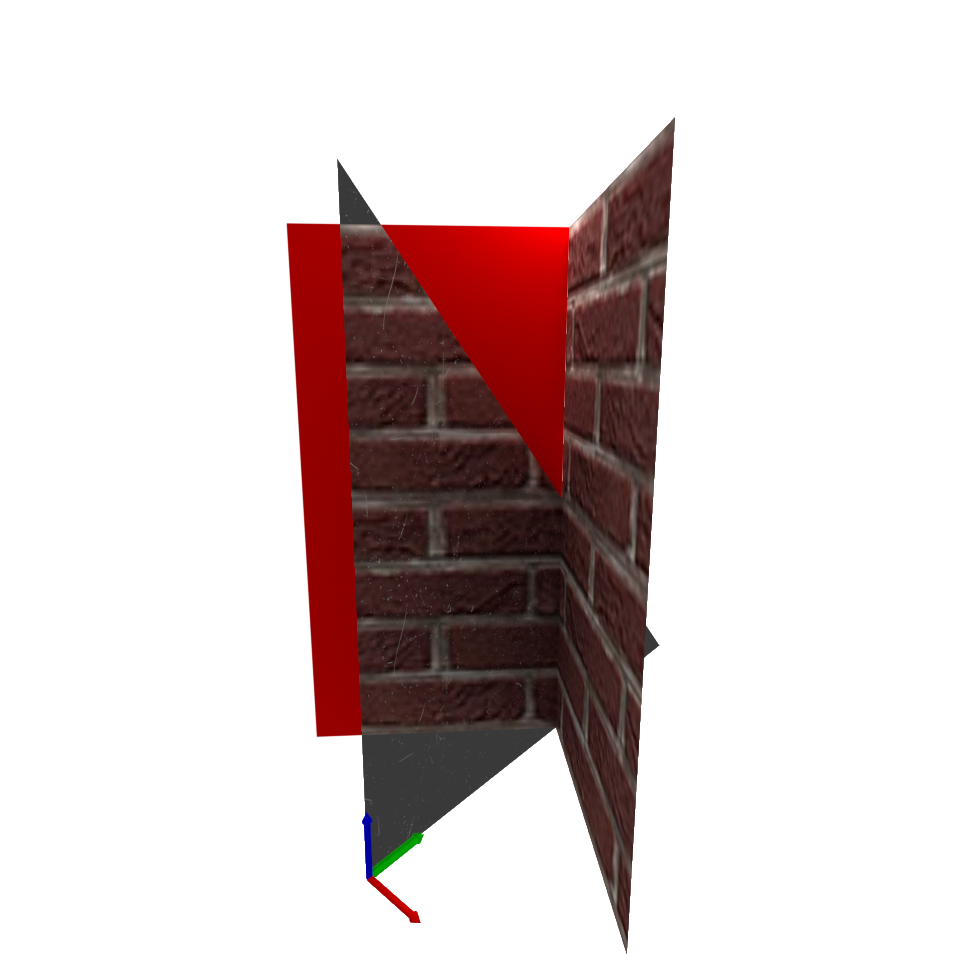
\includegraphics[width=0.45\textwidth]{Reflexion/4}
        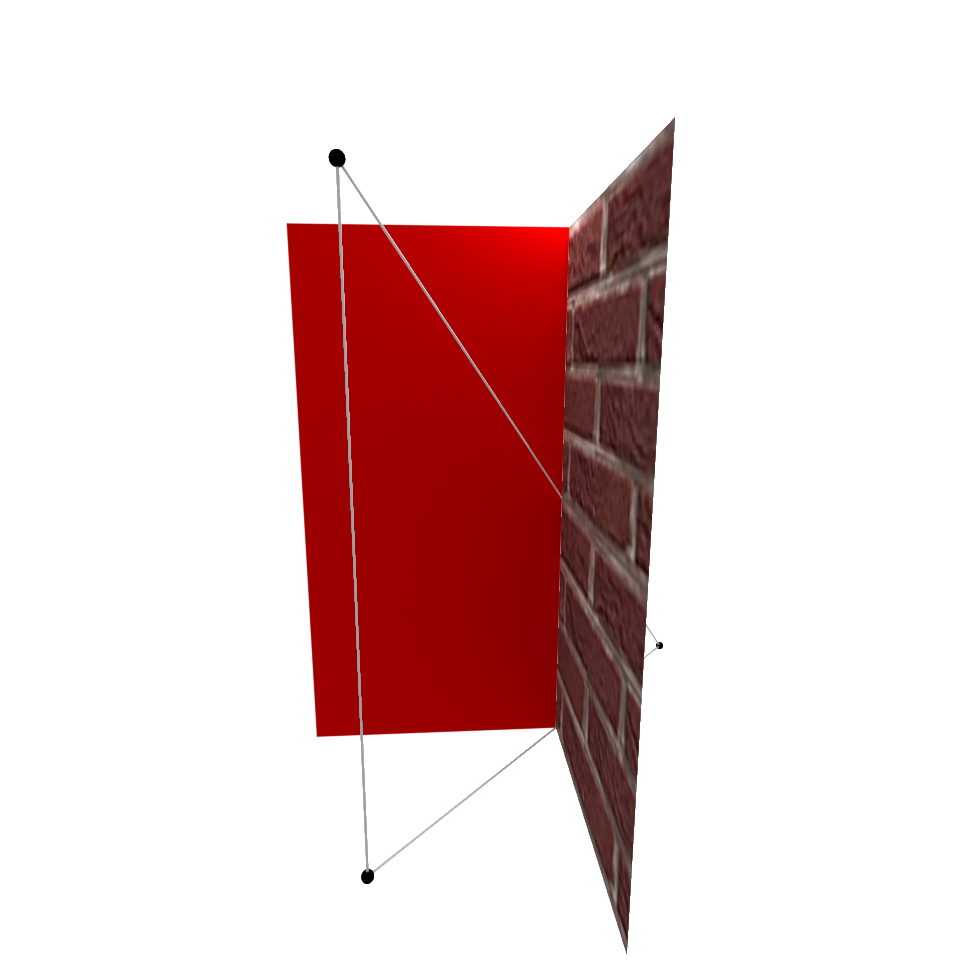
\includegraphics[width=0.45\textwidth]{Reflexion/5}
    \item Et pour finir, on ne garde que les pixels se trouvant à l'intérieur
        du triangle que l'on est en train de rendre.

        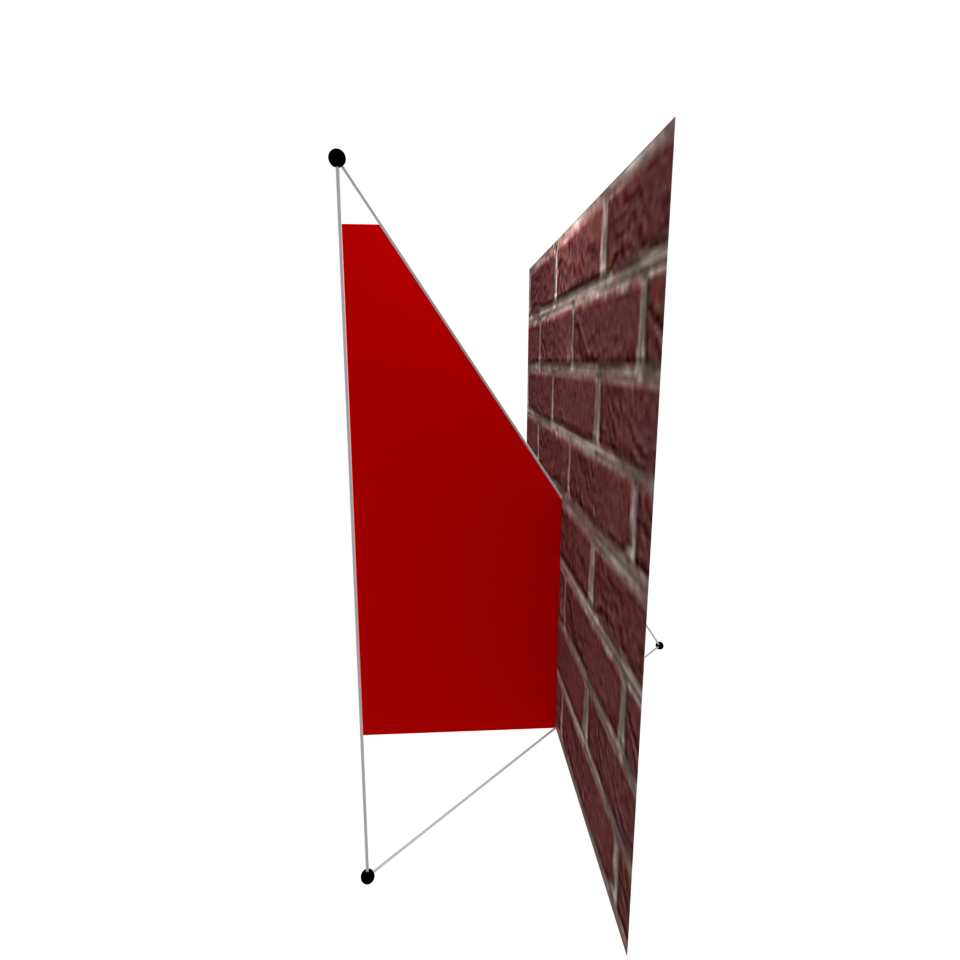
\includegraphics[width=0.45\textwidth]{Reflexion/6}
\end{itemize}

Il reste les réfractions.

Ici, il y a une étape en plus, car la lumière est dispersée, mais aussi décomposée
suivant l'angle d'incidence et le matériau.

On a choisi ici de traiter l'image comme le ferait une vraie caméra~:
en trois canaux de couleur.
On effectue chaque rendu trois fois, ou on rendra de manière séparée, le bleu,
le vert, et le rouge. Chaque réfraction dépendra donc de la matrice TBN de la
surface, de son indice de réfraction, qui est le rapport entre l'angle d'incidence
et l'angle réfracté, et aussi de la longueur d'onde de la couleur
en train d'être rendue.

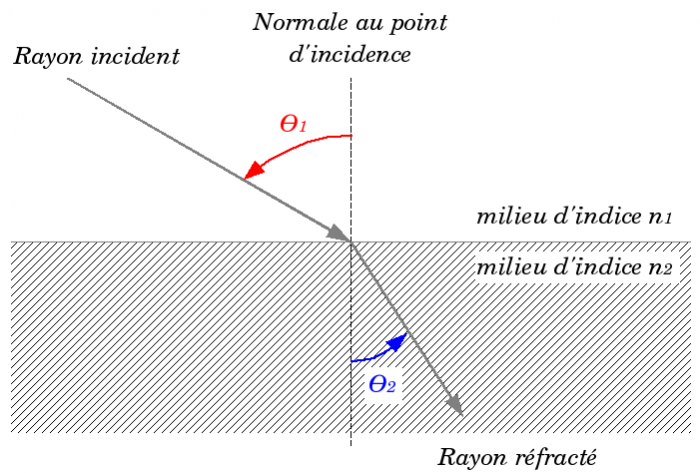
\includegraphics[width=0.65\textwidth]{Refraction/refraction}

Les étapes suivantes sont les mêmes que pour la réflexion.

Ceci étant l'étape triviale de notre algorithme, car il faut maintenant faire la
récurrence afin de voir les réflexions/réfractions sur plusieurs faces (la profondeur
de réflexion étant paramétrable).

Ce n'est pas une étape à prendre à la légère, il faut effectuer un rendu des
réflexions/réfractions pour chaque niveau de récursivité, et ainsi combiner les
textures lors d'un double reflet (Ex: un miroir étant reflété par un autre) en
prenant l'angle d'incidence en compte via l'utilisation du Fresnel.

Cette méthode est très coûteuse en termes de performance,
mais notre but étant le réalisme, cela est satisfaisant.

